
%% bare_conf.tex
%% V1.3
%% 2007/01/11
%% by Michael Shell
%% See:
%% http://www.michaelshell.org/
%% for current contact information.
%%
%% This is a skeleton file demonstrating the use of IEEEtran.cls
%% (requires IEEEtran.cls version 1.7 or later) with an IEEE conference paper.
%%
%% Support sites:
%% http://www.michaelshell.org/tex/ieeetran/
%% http://www.ctan.org/tex-archive/macros/latex/contrib/IEEEtran/
%% and
%% http://www.ieee.org/

%%*************************************************************************
%% Legal Notice:
%% This code is offered as-is without any warranty either expressed or
%% implied; without even the implied warranty of MERCHANTABILITY or
%% FITNESS FOR A PARTICULAR PURPOSE! 
%% User assumes all risk.
%% In no event shall IEEE or any contributor to this code be liable for
%% any damages or losses, including, but not limited to, incidental,
%% consequential, or any other damages, resulting from the use or misuse
%% of any information contained here.
%%
%% All comments are the opinions of their respective authors and are not
%% necessarily endorsed by the IEEE.
%%
%% This work is distributed under the LaTeX Project Public License (LPPL)
%% ( http://www.latex-project.org/ ) version 1.3, and may be freely used,
%% distributed and modified. A copy of the LPPL, version 1.3, is included
%% in the base LaTeX documentation of all distributions of LaTeX released
%% 2003/12/01 or later.
%% Retain all contribution notices and credits.
%% ** Modified files should be clearly indicated as such, including  **
%% ** renaming them and changing author support contact information. **
%%
%% File list of work: IEEEtran.cls, IEEEtran_HOWTO.pdf, bare_adv.tex,
%%                    bare_conf.tex, bare_jrnl.tex, bare_jrnl_compsoc.tex
%%*************************************************************************

% *** Authors should verify (and, if needed, correct) their LaTeX system  ***
% *** with the testflow diagnostic prior to trusting their LaTeX platform ***
% *** with production work. IEEE's font choices can trigger bugs that do  ***
% *** not appear when using other class files.                            ***
% The testflow support page is at:
% http://www.michaelshell.org/tex/testflow/



% Note that the a4paper option is mainly intended so that authors in
% countries using A4 can easily print to A4 and see how their papers will
% look in print - the typesetting of the document will not typically be
% affected with changes in paper size (but the bottom and side margins will).
% Use the testflow package mentioned above to verify correct handling of
% both paper sizes by the user's LaTeX system.
%
% Also note that the "draftcls" or "draftclsnofoot", not "draft", option
% should be used if it is desired that the figures are to be displayed in
% draft mode.
%
\documentclass[conference]{IEEEtran}
% Add the compsoc option for Computer Society conferences.
%
% If IEEEtran.cls has not been installed into the LaTeX system files,
% manually specify the path to it like:
% \documentclass[conference]{../sty/IEEEtran}





% Some very useful LaTeX packages include:
% (uncomment the ones you want to load)


% *** MISC UTILITY PACKAGES ***
%
%\usepackage{ifpdf}
% Heiko Oberdiek's ifpdf.sty is very useful if you need conditional
% compilation based on whether the output is pdf or dvi.
% usage:
% \ifpdf
%   % pdf code
% \else
%   % dvi code
% \fi
% The latest version of ifpdf.sty can be obtained from:
% http://www.ctan.org/tex-archive/macros/latex/contrib/oberdiek/
% Also, note that IEEEtran.cls V1.7 and later provides a builtin
% \ifCLASSINFOpdf conditional that works the same way.
% When switching from latex to pdflatex and vice-versa, the compiler may
% have to be run twice to clear warning/error messages.



\usepackage{fancyhdr}


% *** CITATION PACKAGES ***
%
\usepackage{cite}
% cite.sty was written by Donald Arseneau
% V1.6 and later of IEEEtran pre-defines the format of the cite.sty package
% \cite{} output to follow that of IEEE. Loading the cite package will
% result in citation numbers being automatically sorted and properly
% "compressed/ranged". e.g., [1], [9], [2], [7], [5], [6] without using
% cite.sty will become [1], [2], [5]--[7], [9] using cite.sty. cite.sty's
% \cite will automatically add leading space, if needed. Use cite.sty's
% noadjust option (cite.sty V3.8 and later) if you want to turn this off.
% cite.sty is already installed on most LaTeX systems. Be sure and use
% version 4.0 (2003-05-27) and later if using hyperref.sty. cite.sty does
% not currently provide for hyperlinked citations.
% The latest version can be obtained at:
% http://www.ctan.org/tex-archive/macros/latex/contrib/cite/
% The documentation is contained in the cite.sty file itself.





\usepackage{graphicx}
% *** GRAPHICS RELATED PACKAGES ***
%
\ifCLASSINFOpdf
  % \usepackage[pdftex]{graphicx}
  % declare the path(s) where your graphic files are
  % \graphicspath{{../pdf/}{../jpeg/}}
  % and their extensions so you won't have to specify these with
  % every instance of \includegraphics
  % \DeclareGraphicsExtensions{.pdf,.jpeg,.png}
\else
  % or other class option (dvipsone, dvipdf, if not using dvips). graphicx
  % will default to the driver specified in the system graphics.cfg if no
  % driver is specified.
  % \usepackage[dvips]{graphicx}
  % declare the path(s) where your graphic files are
  % \graphicspath{{../eps/}}
  % and their extensions so you won't have to specify these with
  % every instance of \includegraphics
  % \DeclareGraphicsExtensions{.eps}
\fi
% graphicx was written by David Carlisle and Sebastian Rahtz. It is
% required if you want graphics, photos, etc. graphicx.sty is already
% installed on most LaTeX systems. The latest version and documentation can
% be obtained at: 
% http://www.ctan.org/tex-archive/macros/latex/required/graphics/
% Another good source of documentation is "Using Imported Graphics in
% LaTeX2e" by Keith Reckdahl which can be found as epslatex.ps or
% epslatex.pdf at: http://www.ctan.org/tex-archive/info/
%
% latex, and pdflatex in dvi mode, support graphics in encapsulated
% postscript (.eps) format. pdflatex in pdf mode supports graphics
% in .pdf, .jpeg, .png and .mps (metapost) formats. Users should ensure
% that all non-photo figures use a vector format (.eps, .pdf, .mps) and
% not a bitmapped formats (.jpeg, .png). IEEE frowns on bitmapped formats
% which can result in "jaggedy"/blurry rendering of lines and letters as
% well as large increases in file sizes.
%
% You can find documentation about the pdfTeX application at:
% http://www.tug.org/applications/pdftex





% *** MATH PACKAGES ***
%
%\usepackage[cmex10]{amsmath}
% A popular package from the American Mathematical Society that provides
% many useful and powerful commands for dealing with mathematics. If using
% it, be sure to load this package with the cmex10 option to ensure that
% only type 1 fonts will utilized at all point sizes. Without this option,
% it is possible that some math symbols, particularly those within
% footnotes, will be rendered in bitmap form which will result in a
% document that can not be IEEE Xplore compliant!
%
% Also, note that the amsmath package sets \interdisplaylinepenalty to 10000
% thus preventing page breaks from occurring within multiline equations. Use:
%\interdisplaylinepenalty=2500
% after loading amsmath to restore such page breaks as IEEEtran.cls normally
% does. amsmath.sty is already installed on most LaTeX systems. The latest
% version and documentation can be obtained at:
% http://www.ctan.org/tex-archive/macros/latex/required/amslatex/math/





% *** SPECIALIZED LIST PACKAGES ***
%
%\usepackage{algorithmic}
% algorithmic.sty was written by Peter Williams and Rogerio Brito.
% This package provides an algorithmic environment fo describing algorithms.
% You can use the algorithmic environment in-text or within a figure
% environment to provide for a floating algorithm. Do NOT use the algorithm
% floating environment provided by algorithm.sty (by the same authors) or
% algorithm2e.sty (by Christophe Fiorio) as IEEE does not use dedicated
% algorithm float types and packages that provide these will not provide
% correct IEEE style captions. The latest version and documentation of
% algorithmic.sty can be obtained at:
% http://www.ctan.org/tex-archive/macros/latex/contrib/algorithms/
% There is also a support site at:
% http://algorithms.berlios.de/index.html
% Also of interest may be the (relatively newer and more customizable)
% algorithmicx.sty package by Szasz Janos:
% http://www.ctan.org/tex-archive/macros/latex/contrib/algorithmicx/




% *** ALIGNMENT PACKAGES ***
%
%\usepackage{array}
% Frank Mittelbach's and David Carlisle's array.sty patches and improves
% the standard LaTeX2e array and tabular environments to provide better
% appearance and additional user controls. As the default LaTeX2e table
% generation code is lacking to the point of almost being broken with
% respect to the quality of the end results, all users are strongly
% advised to use an enhanced (at the very least that provided by array.sty)
% set of table tools. array.sty is already installed on most systems. The
% latest version and documentation can be obtained at:
% http://www.ctan.org/tex-archive/macros/latex/required/tools/


%\usepackage{mdwmath}
%\usepackage{mdwtab}
% Also highly recommended is Mark Wooding's extremely powerful MDW tools,
% especially mdwmath.sty and mdwtab.sty which are used to format equations
% and tables, respectively. The MDWtools set is already installed on most
% LaTeX systems. The lastest version and documentation is available at:
% http://www.ctan.org/tex-archive/macros/latex/contrib/mdwtools/


% IEEEtran contains the IEEEeqnarray family of commands that can be used to
% generate multiline equations as well as matrices, tables, etc., of high
% quality.


%\usepackage{eqparbox}
% Also of notable interest is Scott Pakin's eqparbox package for creating
% (automatically sized) equal width boxes - aka "natural width parboxes".
% Available at:
% http://www.ctan.org/tex-archive/macros/latex/contrib/eqparbox/





% *** SUBFIGURE PACKAGES ***
%\usepackage[tight,footnotesize]{subfigure}
% subfigure.sty was written by Steven Douglas Cochran. This package makes it
% easy to put subfigures in your figures. e.g., "Figure 1a and 1b". For IEEE
% work, it is a good idea to load it with the tight package option to reduce
% the amount of white space around the subfigures. subfigure.sty is already
% installed on most LaTeX systems. The latest version and documentation can
% be obtained at:
% http://www.ctan.org/tex-archive/obsolete/macros/latex/contrib/subfigure/
% subfigure.sty has been superceeded by subfig.sty.



%\usepackage[caption=false]{caption}
\usepackage[font=footnotesize]{subfig}
% subfig.sty, also written by Steven Douglas Cochran, is the modern
% replacement for subfigure.sty. However, subfig.sty requires and
% automatically loads Axel Sommerfeldt's caption.sty which will override
% IEEEtran.cls handling of captions and this will result in nonIEEE style
% figure/table captions. To prevent this problem, be sure and preload
% caption.sty with its "caption=false" package option. This is will preserve
% IEEEtran.cls handing of captions. Version 1.3 (2005/06/28) and later 
% (recommended due to many improvements over 1.2) of subfig.sty supports
% the caption=false option directly:
%\usepackage[caption=false,font=footnotesize]{subfig}
%
% The latest version and documentation can be obtained at:
% http://www.ctan.org/tex-archive/macros/latex/contrib/subfig/
% The latest version and documentation of caption.sty can be obtained at:
% http://www.ctan.org/tex-archive/macros/latex/contrib/caption/




% *** FLOAT PACKAGES ***
%
%\usepackage{fixltx2e}
% fixltx2e, the successor to the earlier fix2col.sty, was written by
% Frank Mittelbach and David Carlisle. This package corrects a few problems
% in the LaTeX2e kernel, the most notable of which is that in current
% LaTeX2e releases, the ordering of single and double column floats is not
% guaranteed to be preserved. Thus, an unpatched LaTeX2e can allow a
% single column figure to be placed prior to an earlier double column
% figure. The latest version and documentation can be found at:
% http://www.ctan.org/tex-archive/macros/latex/base/



%\usepackage{stfloats}
% stfloats.sty was written by Sigitas Tolusis. This package gives LaTeX2e
% the ability to do double column floats at the bottom of the page as well
% as the top. (e.g., "\begin{figure*}[!b]" is not normally possible in
% LaTeX2e). It also provides a command:
%\fnbelowfloat
% to enable the placement of footnotes below bottom floats (the standard
% LaTeX2e kernel puts them above bottom floats). This is an invasive package
% which rewrites many portions of the LaTeX2e float routines. It may not work
% with other packages that modify the LaTeX2e float routines. The latest
% version and documentation can be obtained at:
% http://www.ctan.org/tex-archive/macros/latex/contrib/sttools/
% Documentation is contained in the stfloats.sty comments as well as in the
% presfull.pdf file. Do not use the stfloats baselinefloat ability as IEEE
% does not allow \baselineskip to stretch. Authors submitting work to the
% IEEE should note that IEEE rarely uses double column equations and
% that authors should try to avoid such use. Do not be tempted to use the
% cuted.sty or midfloat.sty packages (also by Sigitas Tolusis) as IEEE does
% not format its papers in such ways.





% *** PDF, URL AND HYPERLINK PACKAGES ***
%
%\usepackage{url}
% url.sty was written by Donald Arseneau. It provides better support for
% handling and breaking URLs. url.sty is already installed on most LaTeX
% systems. The latest version can be obtained at:
% http://www.ctan.org/tex-archive/macros/latex/contrib/misc/
% Read the url.sty source comments for usage information. Basically,
% \url{my_url_here}.





% *** Do not adjust lengths that control margins, column widths, etc. ***
% *** Do not use packages that alter fonts (such as pslatex).         ***
% There should be no need to do such things with IEEEtran.cls V1.6 and later.
% (Unless specifically asked to do so by the journal or conference you plan
% to submit to, of course. )


% correct bad hyphenation here
\hyphenation{op-tical net-works semi-conduc-tor}


\begin{document}
%
% paper title
% can use linebreaks \\ within to get better formatting as desired
\title{Distributed Random Servers with Timed Labels for Synchronization over Named Data Network}


% author names and affiliations
% use a multiple column layout for up to three different
% affiliations
\author{\IEEEauthorblockN{Hebi Li, Xiaobin Tan, Zijian Zhou, Zhifan Zhao}
\IEEEauthorblockA{
CAS Key Laboratory of Technology in Geo-spatial Information Processing and Application System\\	
University of Science and Technology of China\\
Hefei, P.R. China\\
Email: lihebi@mail.ustc.edu.cn, xbtan@ustc.edu.cn, zjzhou62@mail.ustc.edu.cn, zzfan@mail.ustc.edu.cn}
}

% conference papers do not typically use \thanks and this command
% is locked out in conference mode. If really needed, such as for
% the acknowledgment of grants, issue a \IEEEoverridecommandlockouts
% after \documentclass

% for over three affiliations, or if they all won't fit within the width
% of the page, use this alternative format:
% 
%\author{\IEEEauthorblockN{Michael Shell\IEEEauthorrefmark{1},
%Homer Simpson\IEEEauthorrefmark{2},
%James Kirk\IEEEauthorrefmark{3}, 
%Montgomery Scott\IEEEauthorrefmark{3} and
%Eldon Tyrell\IEEEauthorrefmark{4}}
%\IEEEauthorblockA{\IEEEauthorrefmark{1}School of Electrical and Computer Engineering\\
%Georgia Institute of Technology,
%Atlanta, Georgia 30332--0250\\ Email: see http://www.michaelshell.org/contact.html}
%\IEEEauthorblockA{\IEEEauthorrefmark{2}Twentieth Century Fox, Springfield, USA\\
%Email: homer@thesimpsons.com}
%\IEEEauthorblockA{\IEEEauthorrefmark{3}Starfleet Academy, San Francisco, California 96678-2391\\
%Telephone: (800) 555--1212, Fax: (888) 555--1212}
%\IEEEauthorblockA{\IEEEauthorrefmark{4}Tyrell Inc., 123 Replicant Street, Los Angeles, California 90210--4321}}




% use for special paper notices
%\IEEEspecialpapernotice{(Invited Paper)}




% make the title area
\maketitle

\lhead{Submitted to INFOCOM'2014 Workshop on Name-Oriented Mobility on 12/30/2013}
\thispagestyle{fancy}

\begin{abstract}
%\boldmath
	Key problem of multi-user real-time communication applications, such as group chat and video conference, is how to synchronize messages among all participants. In this paper, we propose a new protocol based on Named Data Network to address this problem. In this protocol, the system will randomly select multi-level servers in charge of the synchronization of time-labeled control messages, while data fetching in distributed way. This method synthesizes the powerful control ability of servers and NDN's distributed features. We implemented our design and it proved high quality performance of fast data fetching and strong control ability.
\end{abstract}
% IEEEtran.cls defaults to using nonbold math in the Abstract.
% This preserves the distinction between vectors and scalars. However,
% if the conference you are submitting to favors bold math in the abstract,
% then you can use LaTeX's standard command \boldmath at the very start
% of the abstract to achieve this. Many IEEE journals/conferences frown on
% math in the abstract anyway.

% no keywords




% For peer review papers, you can put extra information on the cover
% page as needed:
% \ifCLASSOPTIONpeerreview
% \begin{center} \bfseries EDICS Category: 3-BBND \end{center}
% \fi
%
% For peerreview papers, this IEEEtran command inserts a page break and
% creates the second title. It will be ignored for other modes.
\IEEEpeerreviewmaketitle



\section{Introduction}
% no \IEEEPARstart
% You must have at least 2 lines in the paragraph with the drop letter
% (should never be an issue)
Applications dealing with multi-user communications, like group chat and video conference, is an important part of modern life. However, it is still a problem about how to synchronize data within participants. Traditionally in IP-based network, all the participants should register on the central server, send self-generated messages to the server as well as fetching data back from it. Due that IP-based network only provides support for end-to-end communication, so everyone should set up a connection with the server. The server has to send a copy to every participant regardless of the fact that they may be near each other very much in the topology, resulting in performance problems, such as high burden of links and bandwidth, extremely big overhead, etc. As one of the Future Internet Architecture(FIA)\cite{FIA}, Named Data Network(NDN)\cite{NDN001} goes over the basic downsides of IP-based network, providing the basis of this new method to handle synchronization problems. In NDN, routers will filt the duplicated interest, only send one copy to the next hop, which ensures that there is only one same interest per link. The router will record all the incoming interest's interfaces, so that it could forward the received data to every interface that comes the interest. Besides, NDN router has the ability to cache data packet thanks to Content Store. So if there comes a same interest, the router could satisfy it immediately without fetching for the same data packet again from the producer. The proposed method in this paper take fully advantage of these useful features provided by NDN. In the mean while, this method uses self-generated multi-level servers to synchronize control messages, which is a mix of merits of traditional mode and NDN.

In the very beginning, everyone waits for a specific random time before sending \emph{Any Server Interest} inquiry. If he doesn't receive a reply, he will assume himself the server, and thus ready to satisfy the same interest from others. On receiving this reply, a node will set his server and request control messages from the server. In the case that the region is large, an upper level server will be generated from the lower level servers in the same way, resulting in multi-level architecture. Everyone send a heart beat interest to his server to check whether the server is still available. Once the server failure is detected, a new server that substitutes him will be selected from the clients in the same group. A new participant can find a server to get synchronization control messages in his neighborhood.

When a participant generates some data, he will send interest together with the true data name to inform his server about it. When the server received such interest, he will add his name and time to the label of this record and save it in local log. If there is an upper level server, he will inform his server again in the same way. 

In order to get latest control messages, every participant sends sync interest, which we call \emph{Anything New Interest}, to its server, with the latest labels he knows. When the sync interest times out, a same interest is resent. On receiving the sync interest, the server compares the label with his own. If the label's time is the same as his, it is saved as pending interest for the sake of immediate reply when status updates. If the label is older than his latest label, he will find all the new records after the specific time and send them back in data packet. On receiving this data packet, the client extracts the record from the packet, adds them into his own record log and sends data interest for real data. If the client is also a server in a lower level, he will reply to his client's sync interest, thus forward the synchronization control messages to the whole system.

As for real data fetching, since that the name of every piece of data is stable, the interest from every participant for the same data will be aggregated by routers ensuring no duplicated interests in one link. When the data packet is returned from the publisher, it travels the reverse path of the interest to all the receiver, resulting in small overhead. Besides, the data packet can be cached in router's Content Store, so when there is another participant requesting for the same data, he will get it in the router instead of the publisher.

Our Contribution includes: (1) proposed a new protocol handling the problem of multi-user application synchronization over NDN. (2) implemented our new thoughts on ndnSIM\cite{ndnSIM}. (3) evaluated the performance of our methods. Demonstrated the merits of our design in comparison to another related protocol \emph{ChronoSync\cite{ChronoSync}}.

%Our Contribution includes:
%\begin{enumerate}{\IEEEsetlabelwidth{12}}
%	\item proposed a new protocol handling the problem of multi-user application synchronization over NDN.
%	\item implemented our new thoughts on ndnSIM\cite{ndnSIM}.
%	\item evaluated the performance of our methods. Demonstrated the merits of our design in comparison to another related protocol \emph{ChronoSync\cite{ChronoSync}}.
%\end{enumerate}

The rest of the paper is organized as follows. We describe our protocol design in detail in section \ref{design}. In section \ref{implementation}, we talk about the implementation on ndnSIM over NS3 platform and evaluate the performance. Section \ref{related_work} shows related work, and we conclude the paper in section \ref{conclusion}.

\section{Protocol Design}
\label{design}
\subsection{NDN Background}
This section briefly goes through the necessary Named Data Network architecture background in support for our protocol. In NDN, communication is consumer driven, which means the consumer sends interest to fetch the data back. Every piece of data is specified by its name. When a router receives an interest, it will first check whether the desired data is in its \emph{Content Store(CS)}. If the data packet is already cached in Content Store, the router will drop the interest and return the data packet. If not, the router checks the \emph{Pending Interest Table(PIT)}. In the case the record for this interest is in a router's PIT, the router simply drops the interest and adds an interface to this PIT record. Otherwise the router will finally check the \emph{Forwarding Interest Table(FIB)} by means of \emph{Longest Prefix Match} to determine which interface to forward the interest to. When it still can't find the right way to forward the interest, it drops the interest.

When the publisher receives the interest for his data, he will send the data packet with the same name. On receiving a data packet, the router will check its PIT to see which interface comes the interest for this data. When found, the router forwards the data packet to all the interfaces in the PIT corresponding to the data name and then deletes this PIT record. After that, the router will cache the data packet in its Content Store so that it can satisfy the interest for the same data in the future. In the case that there is no record in the PIT for this data, it means that no one sends the interest for this data or the interest timed out, so it can cache the data packet in its Content Store or just simply drop it. In this way, data packets will be forwarded back to all the consumers in the reverse path of interest packets.

\subsection{Naming Rules}
% \caption command should come BEFORE the table. Table text will default to
% The \label must come after \caption as always.
Naming is one of the most important parts of NDN applications. In this section, we briefly go through all the interest names that we use in this design, and they will be discussed throughly in the following sections for details.

There are four interest names in our design, as in Table \ref{interest_name}. \emph{Any Server Interest} is used for server generation. \emph{Something New Interest} and \emph{Anything New Interest} are responsible for synchronizing control messages. \emph{Data Interest} serves for actual data fetching. The first part is used for router to forward the interest packet correctly. \emph{`/broadcast'} interest is routed to all the corresponding interfaces. \emph{`/serverName'} and \emph{`/publisher'} are routed to specific nodes. The second component, \emph{`/drsapp'} is a specific label for the application.\footnote{To inserting FIBs into routers, the client publishes the interest name, declaring that they can reply to such interest. The router protocols, such as OSPF\cite{OSPF}\cite{OSPFN}, are responsible to inform the other routers this information. ndnSIM provides a function to set the global scale routing FIBs for every node, so in our simulation, we use this to simulate this action}
% It has two functions. The first one is to determine which application is responsible for processing this interest. NDN packet doesn't need to contain a port number as in IP network, so the receiver of the interest use their specific names to hand the interest to the right program. The other purpose of \emph{`/drsapp'} is to optimize the forwarding of a broadcast interest. By default the broadcast interest is forwarded to all the interfaces by a router, which is potential for an interest flooding problem. For example, in actual environment, there may be 100 users connected to a single router, with only 20 of them using this DRSTL application. In such case, the router needs only broadcasting the interest to these 20 people instead of all of them. Remember that NDN router forwards the interest by longest prefix match, so we can add \emph{`/broadcast/drsapp'} in the router to point out the interfaces corresponding to the 20 users.\footnote{This action should be done by the applications on the end node. The client publishes this interest name, declaring that they can reply to such interest. The router protocols, such as OSPF\cite{OSPF}\cite{OSPFN}, are responsible to inform the other routers this information. ndnSIM provides a function to set the global scale routing FIBs for every node, so in our simulation, we use this to simulate this action} In this way, forwarding the broadcast interest is also efficient.

Other components of the names are specified by the procedures, and we will cover them in the following sections in detail.
\begin{table}[!t]
\renewcommand{\arraystretch}{1.3}
\caption{Interests' Names}
\label{interest_name}
\centering
\begin{tabular}{|c|c|}
\hline
Any Server Interest & /broadcast/drsapp/anyserver/\emph{level}\\
\hline
Something New Interest & /\emph{serverName}/drsapp/somethingnew/\emph{mylabel}/\emph{dataName}\\
\hline
Anything New Interest & /\emph{serverName}/drsapp/anythingnew/\emph{label1:label2:label3}\\
\hline
Data Interest & /\emph{publisherName}/drsapp/\emph{time}\\
\hline
\end{tabular}
\end{table}

\subsection{Server Generation}
\begin{figure}[!t]
\centering
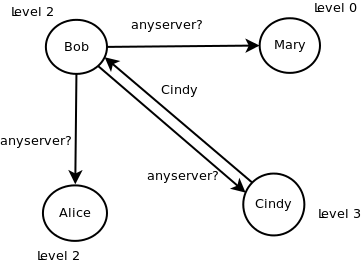
\includegraphics[width=2.5in]{../png/server-generation.png}
\caption{Server Generation}
\label{server_generation}
\end{figure}
To generate servers, the \emph{Any Server Interest} is used. The first two components of the name is used for router forwarding and interest handling. The third one is the interest type. The last element \emph{`level'} is a number indicating in which level the sender currently is.

In the very beginning, everyone doesn't have a server. They will individually wait for a random time and broadcast \emph{Any Server Interest} to inquire whether there is a server nearby. Then they wait a time $T_s$ for the reply. On receiving the data containing the server name, the participant will set his server to this server name and request for synchronization control messages from then on. Otherwise, if he doesn't receive a data after Ts, he assumes himself as the server and thus is ready to reply the such interests from others. 
When the region is large, there should be many groups, each has a selected server. These servers will obey the same rules, wait for a random time, and broadcast an \emph{Any Server Interest} with their current level. After sending this interest, the sender waits a time related to his current level \footnote{This time is a function of current level, because the higher the level is, the larger its region should be, the longer wait time for Any Server Inquiry will be. So the wait time can control the region's area for a particular level. In implementation, interest sender ignores data packet received after this time. However, it is better to support to set the interest life time(hop count) in the low level so that there will not be extra interest sending to unreachable areas.} for the data. If he doesn't receive it after the time expire, he increase his level. The one who receives this interest will compare this level with his own. If this one is lower, he will send data packet to satisfy this interest. 
We can set a small constant number as the Top Level. Whenever a participant has not a server and he is not a top level server, he will act as above in server generation period. If a participant already has a server, he sends heart beat interest to his server to detect possible failure. We will cover failure reversion in Section \ref{trouble_shooting}.

Noting that the server generation procedure is closely related to the reply delay, so the randomly selected multi-level servers are closely related to the topology as well. The direction of transmission is related to the topology, thus it is smart enough not to forward the messages in round. This provides high performance for transferring synchronization control messages between clients and servers.

\subsection{Data Structure}
\begin{figure}[!t]
\centering
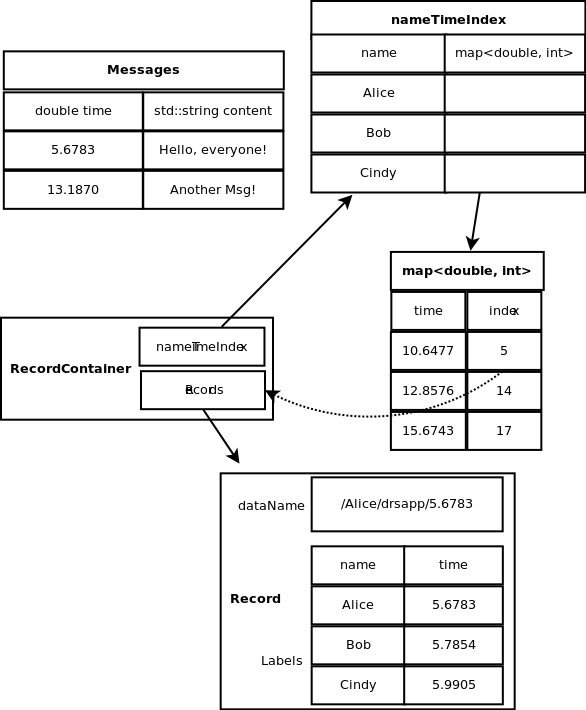
\includegraphics[width=2.5in]{../png/data-structure.png}
\caption{Data Structure}
\label{data_structure}
\end{figure}
In this section, we describe the data structure used for storing and processing synchronization messages.

As shown in Figure \ref{data_structure}, there are two data structures in every node, namely Message Container and Record Container.
Message Container stores the actual data generated by this participant. Keep in mind that participant doesn't need to store everyone else's messages. They only care about whether they have received all the others' messages. However, it is the publisher's responsibility to store his own published messages for the sake of replying the actual data request interest from others.
Record Container holds the synchronization control records. A timed label is the pair of a user name and his time. A record holds a data name and all the labels on behalf of the dataname. A record container consists of two parts, namely \emph{Record Vector} and \emph{NameTimeIndex}. The \emph{Record Vector} is an array of the records by sequence, so that their indexes can tell which is newer. The \emph{NameTimeIndex} structure is a dual map. It is use to find the first index that is newer than a provided label contains a name and time. The index is the one that used in \emph{Record Vector}.

Note that every label about a record contains a user name and user time, thus there's no problem when different participants use different time criteria. Also, since that the record only contains labels from the participants' upper-level servers, and the top level is a small constant number, we don't need to worry about a huge amount of labels. What's more, when a server is down, his labels will never be updated again, so we can use some algorithm like Least Recent Use(LRU)\cite{LRU} to delete useless labels. One more thing, this design provide support for node failure and node mobility, which is referred in Section \ref{mobility}.

\subsection{Synchronization}
\begin{figure}[!t]
\centering
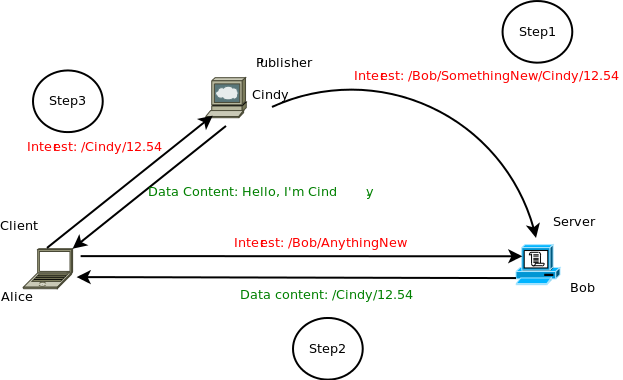
\includegraphics[width=2.5in]{../png/synchronization.png}
\caption{Synchronization and Data Fetching}
\label{synchronization}
\end{figure}
\begin{figure}[!t]
\centering
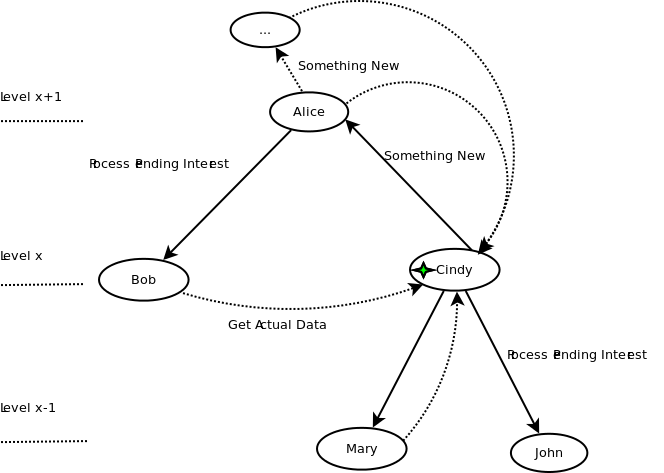
\includegraphics[width=2.5in]{../png/tree-synchronization.png}
\caption{Multi-Level Synchronization}
\label{tree_synchronization}
\end{figure}
We describe how to synchronize in the system in this section. As shown in Figure \ref{synchronization}, a client sends \emph{Something New Interest} to inform server a new change. Server then reply pending \emph{Anything New Interest} with the new change. Participants fetch actual data in distributed way. Figure \ref{tree_synchronization} shows multi-level synchronization. A node will transfer the new status to upper and down level, through sending \emph{Something New Interest} and replying \emph{Anything New Interest} respectively.

\subsubsection{Something New Interest}
Once a node generates a new message, or he receives a \emph{Something New Interest} from his client, he will send this interest to his server with the actual data name.
When a participant generates a new data, he will do the following things:
(1) adds the data to his Message Container.
(2) adds his own label to the record and stores it in his local Record Container.
(3) sends \emph{Something New Interest} with his label and the actual data name to his server
(4) processes pending interest.
On receiving a \emph{Something New Interest}, a server  will do the following things:
(1) removes the labels in this record \footnote{because every node only keeps the labels from his upper level servers.}, add his own label and store it into local Record Container.
(2) sends Something New Interest with his label and the actual data name to his server, if has.
(3) processes pending interest
(4) sends interest with the data name to fetch actual data.

Note that \emph{Something New Interest} contains the actual data name in the end, so once receiving this interest, a node can immediately send this status change to upper and lower level without extra delay.

\subsubsection{Anything New Interest}
To get synchronization control records, every node sends periodically \emph{Anything New Interest} to his server with the newest label on behalf of his status.
When a server receives this interest, he compares the carried label with his own latest label. There are three cases here:
(1) The received label is the same as his own. In such case, he saves this interest as pending interest, so that he can reply immediately when his status changes.
(2) The received label is older than the his own. In this manner, he compares the record's time and find the first index in the Record Container that is newer than the given label. Then he sends back the new records.
(3) There is not any record in his Record Container that shares the same user name as the received label. In this situation, the server has to send back all the records for synchronization.
When the client receives data for Anything New Interest, he will do the following things:
(1) extracts records from the data.
(2) updates his own Record Container.
(3) processes pending interest.
(4) sends data interest to fetch real data.

In general, a server is in charge of inner group synchronization, so every record in the group contains a label of the server. So in regular case, the clients only send his server's latest label. When the system is stable and all nodes share the same status, all \emph{Anything New Interest}s are the same and thus they can be aggregated by NDN routers. Data back can transmit efficiently along the reverse path of interest. When a node moves to another place or the server fails, the node will connect to a new server. In this situation, the last server's label is of no use, so he sends all the latest labels to the new server representing his status. This model can provide natural support for robustness and mobility, which will be covered in section \ref{mobility}. Useless out of date labels will be deleted by some algorithm such as LRU.

\subsection{Distributed Actual Data Fetching}
The servers are only in charge of synchronizing control records, in other words the servers tell the participants in the group when and where to fetch a data. Actual data fetching is acted in distributed way. This design minimizes the messages that travel between server and client, and takes fully advantages of NDN's distributed features such as interest aggregation and caches.

When receiving \emph{Something New Interest} or \emph{Anything New Data}, a participant updates his \emph{Record Container} and send \emph{Data Interest} to fetch actual data. As described above, everyone stores his self-generated data for the sake of replying others' data fetching interest. They don't need to store the fetched data from others, because they only care about whether they have received it or not.


\subsection{Robustness and Mobility Support}
\label{mobility}
\begin{figure}[!t]
\centering
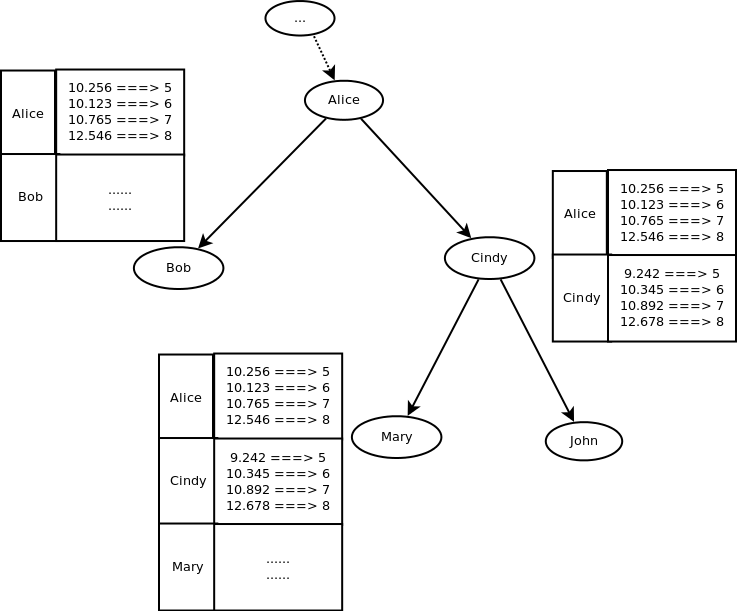
\includegraphics[width=2.5in]{../png/mobility.png}
\caption{Robustness and Mobility Support}
\label{mobility_pic}
\end{figure}
Our proposed model can provide natural robustness and mobility support. When a node goes off-line and returns after some time and connects to the same server, he will send his latest status, which can be recognized easily by the server, since that the server can just compare the time in the label with his own record numerically, find all the new one, and reply to the client. When a node move, whether it is caused by link failure, server failure or the actual move in topology, there are three situations.
(1) he moves to another place, but connects to the same server. In this manner, he can communicate with the server and fetch new things without any affection.
(2) he moves to another place, but connects to a different server. Chances are that he and the new server share a same upper level server \footnote{actually the Top Level Server is always shared by the nodes, but chances are high that a shared upper level server not far away is available because server selection is closely related to topology.}. Although he could not use his former server's labels to communicate with the new server, he can use the shared upper level server's labels with the same performance.
For instance, as shown in Figure \ref{mobility_pic}, assume that Mary moves close to Bob and connects to him. She can not use her former server, Cindy's label now. However, she and Bob hold Alice's label together, thus Bob can still recognize her.
(3) When the node is moved to a completely new environment that even the Top Level Server is not the same. This may be caused by contemporary partition or permanent one, which means the two groups never connect to each other. This situation is extreme, and the node has to exchange all the messages. However, in deed it is not reasonable to handle this condition.

\subsection{Trouble Shooting}
\label{trouble_shooting}
Clients send heat beat interest to detect connection failure. When detected, the client will reset his server and enter server generation period. There are two situations here, the server is down and the client is down. In the first manner, the server is off-line, so the clients in the group will soon select another one to substitute him after the detection. If there are higher level servers, the newly selected server will surely connect to the upper server by sending another \emph{Any Server Interest} with a bigger level, reverting the system to stable architecture. In the second manner, we consider a more general condition that a small group disconnected with the outside world for a while. The participants inside the group can still communicate with each other in this case, and the highest level server in this group will grow to be a \emph{Top Level Server}. When the connection heals, the group should be able to connect to the outside world again and exchange messages instead of remaining a close system with its own \emph{Top Level Server}. To solve this problem, a server can broadcast an interest inquiring if there is a same level server nearby. If so, the server will decrease his level, set his server to the newly detected server and tell his client to connect to the new server too.

\section{Implementation and Evaluation}
\label{implementation}
%Overview goes here
We implemented our protocol on ndnSIM, an overlay of Network Simulation 3(NS3)\cite{ns3}. As a comparison, we implemented another new protocol handling status synchronization problem, the ChronoSync. This section, we will first confirm the rightness of the logic. Then we will evaluate the performance on both packet overhead and delay.

\begin{figure}[!t]
\centering
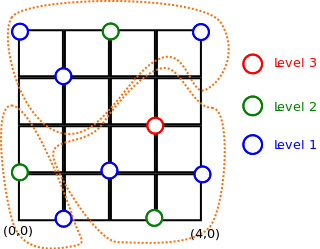
\includegraphics[width=2.5in]{../png/paper-topo.png}
\caption{5x5 Grid Topology and Generated Servers}
\label{paper_topo}
\end{figure}
To be more general, We use the 5x5 grid topology in our simulation, as shown in Figure \ref{paper_topo}. Every node in the grid represents a participant in the synchronization system, thus there are totally 25 nodes. The server is randomly selected, as described before. All links are symmetrical with link delay of 10ms and 1Mbps bandwidth. We let participants randomly generate data, and we change the frequence of the generation to see the trend. Everyone's message generation period is independent.

\subsection{Functional Correctness}
\begin{figure}[!t]
\centering
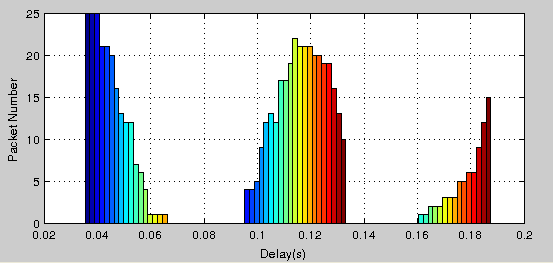
\includegraphics[width=2.5in]{../png/function-delay.png}
\caption{Delay for every node to receive data}
\label{function_delay}
\end{figure}
\subsubsection{Server Generation} In the grid topology, the server generation works well. There forms a four-level architecture, with the top level server on node(3,2). The formed architecture should be better if the topology is random, not symmetrical.

\subsubsection{Message Synchronization} All messages are successfully transfered to every participants. Figure \ref{function_delay} shows the delay of the packages at the frequence of $\frac{2}{7}$Hz. From the graph, we can see that delay is divided into three parts, one very quickly, one average, and the other is a little slow. That is related to the level architecture. If the receiver is close to the publisher in level topology, he should get the message quickly and sends out real data interest. However, in the case that these two participants are far away in the hierarchy tree(chances are high that they are far from each other in the topology too), the synchronization control messages should go through several servers to reach to the other, resulting the delay.

\subsection{Evaluation}

\subsubsection{Overhead}
\begin{figure}[!t]
\centering
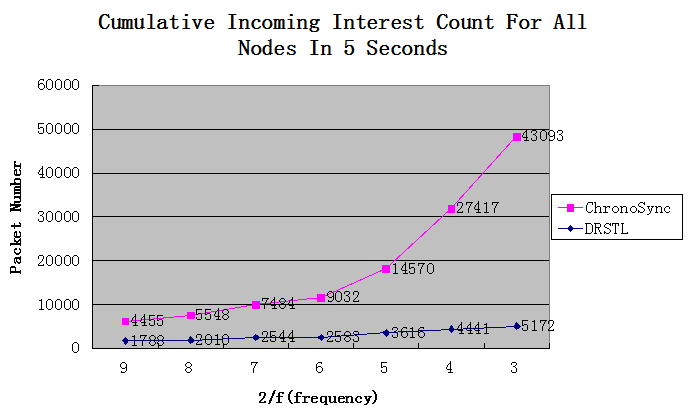
\includegraphics[width=2.5in]{../png/all-incoming-interest.png}
\caption{Incoming Interest Count for All the Nodes}
\label{overhead}
\end{figure}
\begin{figure}[!t]
\centering
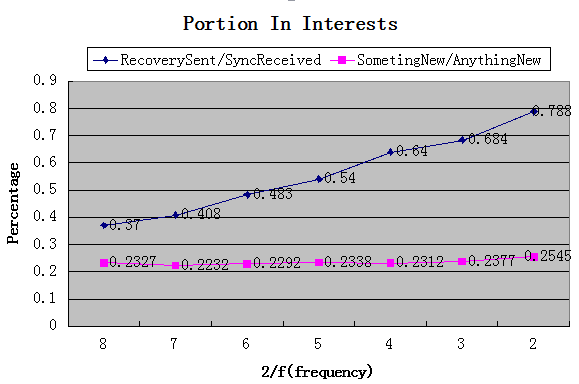
\includegraphics[width=2.5in]{../png/portion-in-interests.png}
\caption{Portion in Interests}
\label{recovery_percentage}
\end{figure}
Our model holds advantage for control, thus the overhead is small. In this experiment, we change the data generation speed and see the overhead change. As shown in Figure \ref{overhead}, as the frequency enhances, our design holds a linear increase in packet delivery count, while ChronoSync suffers a big increase as the frequency goes up, because when the participants generate message more quickly, chance of simultaneous data generation will increase, resulting in ChronoSync applications send out recovery interests to solve the problem. Note that we use all \emph{Incoming Interest}s, because it can represent to the status. The aggregation of NDN router will decline \emph{Incoming Interest} count too. From the view of proportion that consists the interests, as you can see in Figure \ref{recovery_percentage}, the percentage that the receiver will eventually send recovery interest when receiving a sync interest is much higher when data generation frequency increase. However, Something New Interest remains the same ratio with Anything New in DRSTL.

\subsubsection{Delay}
Since control messages should go through multi-level servers in our design, in spite that the level is related to topology, the performance is still lower than ChronoSync, in which data always returns along the best way. However, as a sacrifice, when the data is generated frequently, ChronoSync applications should have to send out recovery interests, resulting in a bigger delay. Figure \ref{delay_compare} shows the delay as a function of frequency. In the graph, we can see that the delay is a little bigger than ChronoSync, but is still pretty good. Take the gained high control ability into consideration, the sacrifice is worthy.
\begin{figure}[!t]
\centering
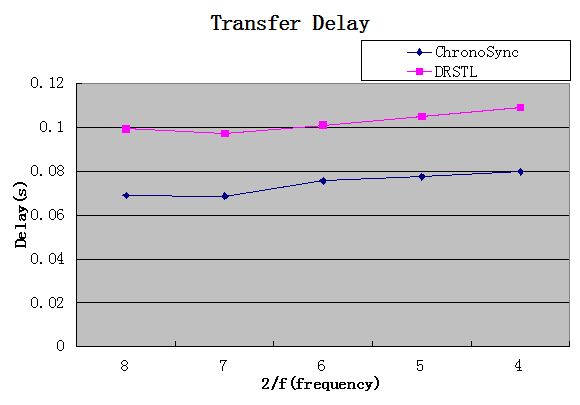
\includegraphics[width=2.5in]{../png/delay-compare.png}
\caption{Delay Compare}
\label{delay_compare}
\end{figure}

\begin{figure}[!t]
\centering
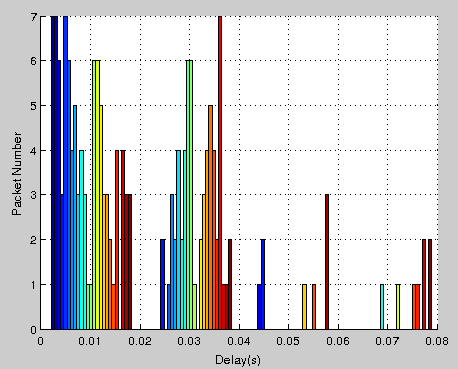
\includegraphics[width=2.5in]{../png/data-fetch-delay.png}
\caption{Data Fetching Delay}
\label{data_fetch_delay}
\end{figure}
Another point, the data fetching procedure is distributed, thus can take fully advantages of NDN architecture. Figure \ref{data_fetch_delay} shows the delay from a participant receives synchronization control message to when he gets the desired data. It is clear that this procedure is very fast, and it contributes to small delay and overhead.

\section{Related Work}
\label{related_work}
Zhenkai Zhu et al recently introduced a new way to handle this problem on NDN, which is an entirely distributed and serverless protocol, named ChronoSync.
In ChronoSync, status is represented using the digest of all participants' current status. Every participant keeps a digest tree and generates the root digest. If all the root digests are the same in the system, then obviously the system status is stable. To recovery from exceptions, every node keeps a digest log that contains the old digest and the trigger events.
Everyone broadcasts a sync interest periodically to the system with its current root digest. Whoever receives a sync interest will compare the digest with his own root digest. If it is the same, he keeps it as a pending digest. If it is in his digest log, he sends back data containing the trigger events. On receiving the data, the receiver knows what data is missing, thus send interest for that piece of data.

Since ChronoSync is entirely distributed, and messages go along the optimized way, it almost has the smallest delay. The main downside of ChronoSync is short of control ability, resulting in problems to handle frequent simultaneous data generation. When this happens, the system will be divided into two different group and can't recognize digest from each other. The solution of ChronoSync is to send recovery interest with the unknown digest. The one who can recognize this digest will send all his current statuses of the whole system back so that the receiver could compare the status with his own to find out what's missing. It should work fine, but in the case that the system is large, or data generation is frequent, video conference for example, there will be lots of simultaneous data generation.

\section{Conclusion}
\label{conclusion}
In this paper, we proposed a new protocol to handle the synchronization problem in multi-user applications. Our design, Distributed Random Servers with Timed Labels, take advantages of both traditional server-based model and NDN's neat and efficient distributed features. (1) Multi-Level servers can provide enough control ability to handle complex conditions; (2) The essential distributed features allow it to fetch data efficiently with little overhead; (3) The hierarchy structure allows the server to control the synchronization by his local time label, which is easy and natural to process compared to using digest. We have implemented our protocol over ndnSIM and evaluated the performance. Data fetching is fast by a distributed way in NDN. With a reasonable delay of sync control message transmission, the overhead is much lower due to powerful control ability. 

Some further topics worth researching include: (1) minimizing within-level delays, (2) generating sever by some better algorithms to generate a hierarchy structure that best fits each specific topology. We will continue focusing on them in the future.

% An example of a floating figure using the graphicx package.
% Note that \label must occur AFTER (or within) \caption.
% For figures, \caption should occur after the \includegraphics.
% Note that IEEEtran v1.7 and later has special internal code that
% is designed to preserve the operation of \label within \caption
% even when the captionsoff option is in effect. However, because
% of issues like this, it may be the safest practice to put all your
% \label just after \caption rather than within \caption{}.
%
% Reminder: the "draftcls" or "draftclsnofoot", not "draft", class
% option should be used if it is desired that the figures are to be
% displayed while in draft mode.
%
%\begin{figure}[!t]
%\centering
%\includegraphics[width=2.5in]{drs3.png}
%\caption{Simulation Results}
%\label{fig_sim}
%\end{figure}

% Note that IEEE typically puts floats only at the top, even when this
% results in a large percentage of a column being occupied by floats.


% An example of a double column floating figure using two subfigures.
% (The subfig.sty package must be loaded for this to work.)
% The subfigure \label commands are set within each subfloat command, the
% \label for the overall figure must come after \caption.
% \hfil must be used as a separator to get equal spacing.
% The subfigure.sty package works much the same way, except \subfigure is
% used instead of \subfloat.
%
%\begin{figure*}[!t]
%\centerline{\subfloat[Case I]\includegraphics[width=2.5in]{drs3.png}%
%\label{fig_first_case}}
%\hfil
%\subfloat[Case II]{\includegraphics[width=2.5in]{drs3.png}%
%\label{fig_second_case}}}
%\caption{Simulation results}
%\label{fig_sim}
%\end{figure*}
%
% Note that often IEEE papers with subfigures do not employ subfigure
% captions (using the optional argument to \subfloat), but instead will
% reference/describe all of them (a), (b), etc., within the main caption.




% Note that IEEE does not put floats in the very first column - or typically
% anywhere on the first page for that matter. Also, in-text middle ("here")
% positioning is not used. Most IEEE journals/conferences use top floats
% exclusively. Note that, LaTeX2e, unlike IEEE journals/conferences, places
% footnotes above bottom floats. This can be corrected via the \fnbelowfloat
% command of the stfloats package.


% conference papers do not normally have an appendix


% use section* for acknowledgement


% trigger a \newpage just before the given reference
% number - used to balance the columns on the last page
% adjust value as needed - may need to be readjusted if
% the document is modified later
%\IEEEtriggeratref{8}
% The "triggered" command can be changed if desired:
%\IEEEtriggercmd{\enlargethispage{-5in}}

% references section

% can use a bibliography generated by BibTeX as a .bbl file
% BibTeX documentation can be easily obtained at:
% http://www.ctan.org/tex-archive/biblio/bibtex/contrib/doc/
% The IEEEtran BibTeX style support page is at:
% http://www.michaelshell.org/tex/ieeetran/bibtex/
%\bibliographystyle{IEEEtran}
% argument is your BibTeX string definitions and bibliography database(s)
%\bibliography{IEEEabrv,IEEEexample}
%
% <OR> manually copy in the resultant .bbl file
% set second argument of \begin to the number of references
% (used to reserve space for the reference number labels box)
\begin{thebibliography}{1}

%\bibitem{IEEEhowto:kopka}
%H.~Kopka and P.~W. Daly, \emph{A Guide to \LaTeX}, 3rd~ed.\hskip 1em plus
%  0.5em minus 0.4em\relax Harlow, England: Addison-Wesley, 1999.
\bibitem{NDN001}
	Zhang, L., Estrin, D., Burke, J., Jacobson, V., Thornton, J. D., Smetters, D. K., ... \& Yeh, E. (2010). Named data networking (ndn) project. Relatório Técnico NDN-0001, Xerox Palo Alto Research Center-PARC.
\bibitem{FIA}
	``NSF Future Internet Architecture Project'', http://www.nets-fia.net
\bibitem{ChronoSync}
	Zhu, Z., \& Afanasyev, A. (2013). Let’s ChronoSync: Decentralized Dataset State Synchronization in Named Data Networking. In Proceedings of the 21st IEEE International Conference on Network Protocols (ICNP 2013).
\bibitem{ndnSIM}
	Afanasyev, A., Moiseenko, I., \& Zhang, L. (2012). ndnSIM: NDN simulator for NS-3. University of California, Los Angeles, Tech. Rep.
\bibitem{ns3}
	``ns-3: a discrete-event network simulator for Internet systems.'', http://www.nsnam.org
\bibitem{OSPF}
	Moy, J. (1998). Open shortest path first (ospf) version 2. IETF: The Internet Engineering Taskforce RFC, 2328.
\bibitem{OSPFN}
	Wang, L., Hoque, A. K. M. M., Yi, C., Alyyan, A., \& Zhang, B. (2012). OSPFN: An OSPF based routing protocol for Named Data Networking. University of Memphis and University of Arizona, Tech. Rep.
\bibitem{LRU}
	Johnson, T., \& Shasha, D. (1994). X3: A Low Overhead High Performance Buffer Management Replacement Algorithm.


\end{thebibliography}


% that's all folks
\end{document}


